%************************************************
% Implementierung
%************************************************
\chapter{Implementierung}
\label{sec:implementation}

In diesem Kapitel wird die Implemetierung des im Rahmen dieser Arbeit entwickelten Programm dargestellt, sowie die technischen Entscheidungen die zu ihr geführt haben, erläutert. Außerdem beschreibt dieses Kapitel die Integration in BlattWerkzeug.

%************************************************
% Objektstruktur
%************************************************
\section{Objektstruktur}
\label{sec:implementation:structure}

\TODO{} wurde zunächst eine Objektorientierte Datenstruktur erarbeitet, die eine Welt repräsentieren und Operationen auf der Welt durchführen kann. \figreft{fig:implementation:structure:uml} zeigt ein UML-Diagram dieser Struktur. Zur besseren Übersicht wurde diese Darstellung auf die wehsentlichen zum Verständnis notwenigen Klassen, Attribute und Operationen beschränkt.

\begin{figure}
  \begin{tikzpicture}
  \tikzstyle{every node}=[font=\small]

  \begin{class}[text width=5cm]{World}{4.75,0}
    \attribute{commands}
    \attribute{sensors}

    \operation{command(command: Command)}
    \operation{sensor(sensor: Sensor): boolean}
  \end{class}

  \begin{class}[text width=3cm]{Size}{-1.5,-1}
    \attribute{width: number}
    \attribute{height: number}
  \end{class}

  \begin{class}[text width=3cm]{WorldState}{11,-1.5}
    \attribute{step: number}
    \attribute{time: number}
    \attribute{prev: WorldState}
  \end{class}

  \begin{class}[text width=4cm]{Tile}{-1,-3.5}
    \attribute{position: Position}
    \attribute{freightTarget: Freight}

    \operation{addFreight(freight: Freight)}
    \operation{removeFreight(): Freight}
  \end{class}

  \begin{class}[text width=5cm]{Truck}{10,-5}
    \attribute{position: Position}
    \attribute{facing: number}

    \operation{loadFreight(freight: Freight)}
    \operation{unloadFreight(): Freight}
    \operation{turn(turnDirection: TurnDirection)}
    \operation{move()}
  \end{class}

  \begin{class}[text width=6cm]{TrafficLight}{4.75,-10}
    \attribute{redPhase: number}
    \attribute{greenPhase: number}
    \attribute{initial: number}

    \operation{isRed(step: number): boolean}
    \operation{isGreen(step: number): boolean}
  \end{class}

  \begin{enumeration}[text width=4cm]{TileOpening}{-1,-8}
    \attribute{None}
    \attribute{North}
    \attribute{East}
    \attribute{South}
    \attribute{West}
  \end{enumeration}

  \begin{enumeration}[text width=3.5cm]{Freight}{4.25,-4.5}
    \attribute{Red}
    \attribute{Green}
    \attribute{Blue}
  \end{enumeration}

  \begin{enumeration}[text width=4cm]{TurnDirection}{10.5,-10.5}
    \attribute{Straight}
    \attribute{Left}
    \attribute{Right}
  \end{enumeration}

  \aggregation{World}{size}{1}{Size}
  \aggregation{World}{states}{*}{WorldState}
  \aggregation{WorldState}{tiles}{*}{Tile}
  \aggregation{WorldState}{truck}{1}{Truck}
  \aggregation{Tile}{trafficLights}{0..4}{TrafficLight}
  \unidirectionalAssociation{Truck}{turning}{1}{TurnDirection}
  \unidirectionalAssociation{Tile}{openings}{1..4}{TileOpening}
  \unidirectionalAssociation{Truck}{freight}{0..*}{Freight}
  \unidirectionalAssociation{Tile}{freight}{0..*}{Freight}
\end{tikzpicture}

  \caption{Vereinfachtes UML-Diagramm der Weltobjektstruktur}
  \label{fig:implementation:structure:uml}
\end{figure}

Wurzelelement dieser Struktur ist die \inlinec{World}-Klasse. Sie wird mit einer Beschreibung der zu genrierenden Welt instanziiert. Anhand dieser Beschreibung erzeugt der Kontruktor die Größe (\inlinec{Size}) der Welt, einen Lastwagen (\inlinec{Truck}) und eine Menge von Kacheln (\inlinec{Tile}). Lastwagen und Kacheln werden in einen Weltzustand (\inlinec{WorldState}) verpackt. Die Daten eines einmal gespeicherten Zustandes werden nicht mehr geändert. Stattdessen wird eine Kopie des aktuellen Zustandes erzeugt, verändert und in die Liste aller Zustände abgespeichert. Dieses Vorgehen wurde gewählt, um dem Nutzer zu ermöglichen Aktionen wieder rückgängig zu machen. Außerdem vereinfacht sie die für die Animationen \tref{sec:implementation:rendering:animation} notwenige Interpolation zwischen Zuständen. Die Veränderung der Zustände übernimmt die \inlinec{World}-Klasse in der Operation \inlinec{command}.

%************************************************
% Programmiersprache
%************************************************
\section{Programmiersprache}
\label{sec:implementation:program}

\TODO{}

\subsection{Elemente der Sprache}
\label{sec:implementation:program:elements}

Im Folgenden sind die Elemente beschrieben, welche dem Nuzter zum Programmieren innerhalb der bereitgestellten Umgebung zur Verfügung stehen.

\subsubsection{Atomare Befehle}
\label{sec:implementation:program:elements:cmds}

Wichtigster Bestandteil sind die \emph{atomaren Befehle}. Durch die Aneinanderreihung mehrerer Befehle lässt sich bereits ein sinnvolles Programm implementieren. Als notwendige Befehle wurden identifiziert:

% \begin{itemize}
%   \item \emph{Vorwärts fahren}: Bewegt den Lastwagen nach Vorne. Falls dabei ein Blinker in eine Richtung gesetzt ist, biegt der Laswagen in die entsprechende Richtung ab.
%   \item \emph{Blinker links setzten}: Setzt den Blinker auf der linken Seite. Dadurch biegt der Lastwagen bei der nächsten Vorwärtsbewegung links ab.
%   \item \emph{Blinker rechts setzten}: Setzt den Blinker auf der rechten Seite. Bei der nächsten Vorwärtsbewegung biegt der biegt der Lastwagen dadurch entsprechend rechts ab.
%   \item \emph{Blinker ausschalten}: Schaltet einen vorher eingeschalteten Blinker wieder aus.
%   \item \emph{Aufladen}: Läd ein Frachstück, welches vor dem Lastwagen liegt auf.
%   \item \emph{Abladen}: Läd ein Frachtstück auf eine Ablagefläche oder einen leeren Steckenabschnitt vor dem Lastwagen wieder ab.
%   \item \emph{Warten}: Wartet einen Zeitschritt ab. Dieser Befehl ist wichtig um das warten auf eine Ampel zu ermöglichen.
% \end{itemize}

\begin{table}[H]
  \begin{tabular}{|p{0.175\textwidth}|p{0.175\textwidth}|p{0.56\textwidth}|}
    \hline
    \textbf{Befehl} & \textbf{Interne\newline Repräsentation} & \textbf{Beschreibung} \\ \hline
    Vorwärts fahren & \inlinec{goForward} & Bewegt den Lastwagen nach Vorne. Falls dabei ein Blinker in eine Richtung gesetzt ist, biegt der Laswagen in die entsprechende Richtung ab. \\ \hline
    Blinker\newline links setzten & \inlinec{turnLeft} & Setzt den Blinker auf der linken Seite. Dadurch biegt der Lastwagen bei der nächsten Vorwärtsbewegung links ab. \\ \hline
    Blinker\newline rechts setzten & \inlinec{turnRight} & Setzt den Blinker auf der rechten Seite. Bei der nächsten Vorwärtsbewegung biegt der biegt der Lastwagen dadurch entsprechend rechts ab. \\ \hline
    Aufladen & \inlinec{load} & Läd ein Frachstück, welches vor dem Lastwagen liegt auf. \\ \hline
    Abladen & \inlinec{unload} & Läd ein Frachtstück auf eine Ablagefläche oder einen leeren Steckenabschnitt vor dem Lastwagen wieder ab. \\ \hline
    Warten & \inlinec{wait} & Wartet einen Zeitschritt ab. Dieser Befehl ist wichtig um das warten auf eine Ampel zu ermöglichen. \\ \hline
  \end{tabular}
  \vspace{5pt}
  \caption{Atomare Befehle}
  \label{tbl:implementation:program:elements:cmds}
\end{table}

Bewegungen finden dadurch immer relativ zur aktuellen Blickrichtung des Lastwagen statt. Dieser Ansatz wurde einem absoluten Ansatz mit Befehlen wie "Fahre nach Norden", "Fahre nach Osten", usw. vorgezogen, da er der intuitiven Steuerungsart eines Lastwagen am nächsten kommt. Außerdem können daraus Vorteile für die Darstellung gewonnen werden \tref{sec:implementation:rendering:truck-position}.

\subsubsection{Zählerschleife}
\label{sec:implementation:program:elements:for}

Um Codeverdoppelung zu vermeiden kann eine \emph{Schleife} eingesetzt werden, die einen Befehlsblock wiederholt. Die Anzahl der Wiederholungen kann vom Nutzer festgelegt werden.

\subsubsection{Sensoren}
\label{sec:implementation:program:elements:sensors}

Um Verzweigungen Nutzen zu können, gibt es die Möglichkeit Werte von \emph{Sensoren} abzufragen. Sensoren stehen immer entweder auf Wahr oder Falsch. Folgende Sensoren stehen zur Verfügung:

% \begin{itemize}
%   \item \emph{Ampel ist rot}: Dieser Sensor ist Wahr, wenn die Ampel vor dem Lastwagen rot ist. Ist, die Ampel grün, oder es gibt keine Ampel vor dem Lastwagen, so steht dieser Sensor auf Falsch.
%   \item \emph{Ampel ist grün}: Ananlog dazu, ist dieser Sensor Wahr, wenn die Ampel vor dem Lastwagen grün ist und Falsch, wenn sie auf rot steht oder es keine Ampel vor dem Lastwagen gibt.
%   \item \emph{Kann geradeaus fahren}: Dieser Sensor wertet zu Wahr aus, wenn das Straßennetz es zulässt, dass der Lastwagen im nächsten Schritt geradeaus fahren kann.
%   \item \emph{Kann links abbiegen}: Dieser Sensor wertet zu Wahr aus, wenn im nächsten Schritt links abgebogen werden kann.
%   \item \emph{Kann rechts abbiegen}: Wenn im nächsten Schritt nach rechts abgebogen werden kann, wertet dieser Sensor zu Wahr aus.
%   \item \emph{Ist gelöst}: Wenn die aktuelle Welt gelöst wurde, also alle Frachtstücke zu ihren Zielen transporiert wurden, wertet dieser Sensor zu Wahr aus.
% \end{itemize}

\begin{table}[H]
  \begin{tabular}{|p{0.175\textwidth}|p{0.175\textwidth}|p{0.56\textwidth}|}
    \hline
    \textbf{Sensor} & \textbf{Interne\newline Repräsentation} & \textbf{Beschreibung} \\ \hline
    Ampel ist rot & \inlinec{lightIsRed} & Dieser Sensor ist Wahr, wenn die Ampel vor dem Lastwagen rot ist. Ist, die Ampel grün, oder es gibt keine Ampel vor dem Lastwagen, so steht dieser Sensor auf Falsch. \\ \hline
    Ampel ist grün & \inlinec{lightIsGreen} & Ananlog dazu, ist dieser Sensor Wahr, wenn die Ampel vor dem Lastwagen grün ist und Falsch, wenn sie auf rot steht oder es keine Ampel vor dem Lastwagen gibt. \\ \hline
    Kann geradeaus fahren & \inlinec{canGoStraight} & Dieser Sensor wertet zu Wahr aus, wenn das Straßennetz es zulässt, dass der Lastwagen im nächsten Schritt geradeaus fahren kann. \\ \hline
    Kann links abbiegen & \inlinec{canTurnLeft} & Dieser Sensor wertet zu Wahr aus, wenn im nächsten Schritt links abgebogen werden kann. \\ \hline
    Kann rechts abbiegen & \inlinec{canTurnRight} & Wenn im nächsten Schritt nach rechts abgebogen werden kann, wertet dieser Sensor zu Wahr aus. \\ \hline
    Ist gelöst & \inlinec{isSolved} & Wenn die aktuelle Welt gelöst wurde, also alle Frachtstücke zu ihren Zielen transporiert wurden, wertet dieser Sensor zu Wahr aus. \\ \hline
  \end{tabular}
  \vspace{5pt}
  \caption{Sensoren}
  \label{tbl:implementation:program:elements:sensors}
\end{table}

\subsubsection{Abweisende Schleife}
\label{sec:implementation:program:elements:while}

Mit den Sensoren ist es möglich eine abweisende Schleife zu nutzen. Diese wiederholt den Befehlsblock solange der angegebene Ausdruck zu Wahr auswertet. Wird die Schleifenbedingung vor der ersten Ausführung des Schleifenblocks oder nach ein oder mehrerer Ausführungen zu Falsch ausgewertet, wird der nächste Blocks ausgeführt. Der Schleifenblock kann also auch komplett übersprungen werden.

\subsubsection{Verzweigungen}
\label{sec:implementation:program:elements:if-else}

Sensoren ermöglichen außerdem Verzweigungen, die einen Befehlsblock nur dann ausführen, wenn der angegebene Sensor zu Wahr ausgewertet wird und einen weiteren, optionalen Befehlsblock, wenn der Sensor zu Falsch ausgewertet wird.

Das aus anderen Sprachen bekannte \inlinec{elseif} gibt es, wie auch in JavaScript, in der hier definierten Sprache nicht. Um dieses Verhalten zu erreichen, müssen mehrere \inlinec{if...else}-Anweisungen geschachtelt werden. In Zukunft wäre es denkbar, in dieser Form geschachtelte Verzweigungen auch im generierten Code ohne zusätzliche geschweifte Klammern und Einrückung darzustellen. Bisher wurde auf diese Darstellung verzichtet, da auch der Drag \& Drop-Editor hierzu noch nicht in der Lage ist.

\subsubsection{Logische Operatoren}
\label{sec:implementation:program:elements:op}

Mit Hilfe von logische Operatoren können neue Ausdrücke erzeugt werden, welche sich wiederum in Schleifen und Verzweigungen einzetzten lassen.

\begin{itemize}
  \item Die \emph{Nicht}-Operation kehrt den Wahrheitswert um.
  \item Die \emph{Und}-Verknüpfung ergibt "Wahr", wenn beide Verküpften Werte "Wahr" sind.
  \item Die \emph{Oder}-Verküpfung ergibt "Wahr", wenn mindestens einer der beiden Verküpften Werte "Wahr" ist.
\end{itemize}

Mit diesen logischen Operatoren ist es nun z.B. möglich zu prüfen, ob das vorrausliegende Steckenstück eine Kurve ist: (Kann nicht geradeaus fahren und ((Kann links abbiegen und Kann nicht rechts abbiegen) oder (Kann nicht links abbiegen und Kann rechts abbiegen)))

\subsubsection{Prozeduren}
\label{sec:implementation:program:elements:proc}

Desweiteren ist es möglich eigene Prozeduren zu definieren und aufzurufen. Für Prozeduren lassen sich zusätzlich Parameter definieren, deren Nutzung innerhalb des Prozedurenblocks möglich ist. Jeder Parameter erhält einen vom Nuzter festgelegten Namen, kann jedoch ausschließlich boolsche Werte übergeben. Bei Aufruf der Prozedur werden die übergebenen Werte -- wie bei Prozeduraufrufen in JavaScript üblich -- kopiert.

Funktionen sind in der Lage sich selbst aufzurufen. Dies ermöglicht zusätzlich die Nutzung von Rekursion. In Verbindung mit Verzweigungen ist auch Rekursion mit Abbruchbedingungen möglich.

\subsection{Auswertung}
\label{sec:implementation:program:evaluation}

Für die Auswertung und Ausführung des durch den Syntaxbaum beschriebenen Code kommen zwei Vorgehensweisen infrage. Im Grundlagenkapitel \ref{sec:basics:compile-interpret} wurde der Unterschied zwischen Kompilieren und Interpretieren im klassischen Sinne bereits erklärt. Da im Browser jedoch nicht direkt Maschienencode ausgeführt werden kann ist der Unterschied in diesem Zusammenhang etwas anders zu verstehen.

\begin{itemize}
  \item Beim \emph{Interpretieren} wird der Syntaxbaum nach und nach durch ein in JavaScript geschriebenes Programm abgearbeitet und die entsprechenden Befehle direkt ausgeführt. In dieser Umgebung lässt sich der Fortschritt des Programms leicht verfolgen, da der Interpreter zu jedem Zeitpunkt die Position kennt bis zu der der Code bisher ausgeführt wurde. Dies ermöglicht den Einbau von Aussagekräftigen Debuggingfunktionen für den den auszuführenden Code. Außerdem ist es leicht möglich Mechanismen bereitzustellen, welche die Ausführung an einer beliebigen Stelle stoppen oder pausieren und später fortsetzen.
  \item Im Unterschied dazu ist \emph{Kompilieren} in diesem Zusammenhang so zu verstehen, dass ein JavaScript-Programm den Syntaxbaum zunächst in einen vollständig ausführbaren JavaScript-Code überführt. Der JavaScript-Code liegt bei diesem Vorgehen nach dem Kompilieren als String vor und kann anschließend als ganzes in einer Art Sandkasten ausgeführt werden. Innerhalb dieser "Blackbox" lässt sich nur recht unzuverlässig auf den aktuellen Zustand des laufenden Programmes schließen ohne zusätzlichen Code code einzufügen, der die Lesbarkeit des generierten Codes verschlechtert. Eben diese Lesbarkeit des generierten Codes ist einer der wichtigsten Vortile dieser Vorgehensweise. Der Code lässt sich nicht nur für seine Ausführung nutzen, sondern kann gerade im Kontext einer Lernsoftware für den Nutzer interessant sein.
\end{itemize}

Im Verlauf der Arbeit wurde die Vorgehensweise "Kompilieren" an dieser Stelle als Anforderung festgelegt, da dieses Vorgehen speziell für BlattWerkzeug den Vorteil mit sich bringt, dass generierter Code in Zukunft vor der Ausführung dem Nutzer angezeigt und von ihm bearbeitet werden kann, was den Übergang zu einer Universalsprache erleichtern würde \TODO{Verweis auf Ausblick}.

\subsubsection{Codegenerator}

Für die Kompilierung des Syntaxbaum wird auf den von BlattWerkzeug zur Verfügung gestellten Codegenerator-Strukturen zurückgegriffen, die es ermöglichen einen Codegenrator zu implementieren, der Übersetzungsregeln für jeden Knotentypen definiert. \figreft{fig:implementation:program:evaluation:while} zeigt die Implementierung eines Codegenrators für Knoten, die eine While-Schleife repräsentieren. Zwischen den Klammern innerhalb der \inlinec{while}-Anweisung wird der Kindknoten für die Bedingung der Schleife eingefügt, gefolgt vom Inhalt der Schleife. Diese Kindknoten werden wiederrum durch ähnlich aufgebaute Generatoren umgewandelt bis der vollständige Code des Wurzelknoten im Syntaxbaum generiert wurde.

\begin{figure}
  \lstinputlisting{snippets/implementation-program-evaluation-while.ts}
  \caption{Beispielhafte Implementierung eines Codegenrator für eine While-Schleife}
  \label{fig:implementation:program:evaluation:while}
\end{figure}

\subsubsection{Syntaxfehler}

Es kann nicht garantiert werden, dass der Code, welcher vom Codegenrator erzeugt wurde, frei von Syntaxfehlern ist. Dies resultiert aus der Kompilierung eines unvollständigen Syntaxbaumes. So kann es z.B. vorkommen, dass die Bedingung bei einer While-Schleife leer ist. JavaScript wirft bei der Erzeugung der Funktion einen \inlinec{SyntaxError}, um diesen Fehler abzufangen, muss die Erzeugung der Funktion in einer try...catch-Anweisung\footnote{\url{https://developer.mozilla.org/de/docs/Web/JavaScript/Reference/Statements/try...catch}} stattfinden \fref{fig:implementation:program:evaluation:try-catch}.

\begin{figure}
  \lstinputlisting{snippets/implementation-program-evaluation-try-catch.js}
  \caption{Möglicher Syntaxfehler innerhalb des generierten Code}
  \label{fig:implementation:program:evaluation:try-catch}
\end{figure}

\subsubsection{Umgebung zur Ausführung}

Dem kompilierten Code muss zur Ausführung eine Umgebung bereitgestellt werden, welche die eingangs als "atomaren Befehele" bezeichneten Funktionen, sowie Funktionen zur Ermittlung der Sensorwerte zur Verfügung stellt. Für diese Aufgabe bietet sich der \inlinec{Function}-Konstruktor\footnote{\url{https://developer.mozilla.org/de/docs/Web/JavaScript/Reference/Global_Objects/Function}} an. Im Gegensatz zu \inlinec{eval} ermöglicht der \inlinec{Function}-Konstruktor die Ausführung von Code im globalen Gültigkeitsbereich, was zu besseren Programmiergewohnheiten führt und eine effizientere Code-Minimierung ermöglicht~\cite{mdn-function}. In diesem speziellen Fall wird für die Ausfühung des Codes der \inlinec{AsyncFunction}-Konstruktor verwendet (siehe dazu \treft{sec:implementation:rendering:animation}).

Für die Bereitstellung der Befehle und Sensoren werden im Folgenden drei Varianten betrachtet. In Abbildung \ref{fig:implementation:program:environment} werden Implementationsbeispiele dieser Varianten gegenüber gestellt.

\begin{enumerate}
  \item Eine Enum-Klasse mit allen Sensoren und Befehlen, sowie zwei Funktionen deren Auswertung, gibt es schon. Darauf aufbauend wäre eine naheliegend Möglichkeit, diese Funktionen und die Enum-Klassen einfach in der Welt bereitzustellen. Ein deutlicher Vorteil dieser Lösung ist der geringe zusätzliche Implementierungsaufwand und die verbesserte Wartbarkeit. Kommen neue Befehle oder Sensoren dazu, stehen diese automatisch auch in der Umgebung zur Verfügung. Der generierte Code ist jedoch nicht intuitiv und sollte er dem Nutzer angezeigt werden, nicht besonders gut zu verstehen. Außerdem halten sich die Funktionsaufrufe nicht an gängige Muster, was den späteren Umstieg auf Universalsprachen erschweren könnte \fref{fig:implementation:program:environment:func}.
  \item Eine weitere denkbare Lösung ist es ein Objekt mit allen benötigten Funktionen für Befehle und Sensoren zu erzeugen und dieses als Wert von \inlinec{this} innerhalb der Funktion zur Verfügung zu stellen. Selbstdefinierte Prozeduren, werden innerhalb der Funktion ebenfalls als Kinder von \inlinec{this} definiert. Dieses Vorgehen hat den Vorteil, dass der Code deutlich intuitiver wird, als dies bei der vorgehend beschriebenen Variante der Fall wäre. Jedem Aufruf muss zwar ein \inlinec{this} vorangestellt werden, jeder Befehl hat aber seinen eigenen Funktionsaufruf. Der zusätzliche Implemetierungsaufwand ist allerdings ein Nachteil dieser Variante. Es müssen in einem Objekt, Wrapper-Funktionen für alle Befehle und Sensoren definiert werden. Kommt zu einem späteren Zeitpunkt ein Befehl oder ein Sensor hinzu, muss dieser zusätzlich auch an dieser Stelle hinzugefügt werden \fref{fig:implementation:program:environment:this}.
  \item Auch wäre es möglich alle Befehle und Sensoren als Parameter der Funktion zu definieren. Dadurch würde im Vergleich zur vorigen Variante die Notwendigkeit entfallen \inlinec{this.} vor jeden Aufruf zu stellen. Da die Wrapper-Funktionen in diesem Fall allerdings ebenfalls zusätzlich definiert werden müssen und die Zuordnung ihrer Namen fehleranfällig ist, birgt dieses Vorgehen abgesehen des etwas kompakteren Codes, keine weiteren Vorteile \fref{fig:implementation:program:environment:param}.
\end{enumerate}

Für die Implementierung scheint Variante zwei am sinnvollsten. Es wird also ein Objekt mit Wrapper-Funktionen für alle Befehle und Sensoren erzeugt und dieses mittels \inlinec{call}\footnote{\url{https://developer.mozilla.org/de/docs/Web/JavaScript/Reference/Global_Objects/Function/call}} an die generierte Funktion übergeben.

\begin{figure}
  \begin{subfigure}[b]{\textwidth}
    \lstinputlisting{snippets/implementation-program-environment-func.js}
    \caption{Definition und Aufruf mit Enum-Klasse}
    \label{fig:implementation:program:environment:func}
    \vspace{0.5cm}
  \end{subfigure}
  \begin{subfigure}[b]{\textwidth}
    \lstinputlisting{snippets/implementation-program-environment-this.js}
    \caption{Definition und Aufruf mit \inlinec|call|}
    \label{fig:implementation:program:environment:this}
    \vspace{0.5cm}
  \end{subfigure}
  \begin{subfigure}[b]{\textwidth}
    \lstinputlisting{snippets/implementation-program-environment-param.js}
    \caption{Definition und Aufruf über Parameter}
    \label{fig:implementation:program:environment:param}
  \end{subfigure}
  \caption{Varianten für die Bereitstellung der Befehle und Sensoren innerhalb der generierten Funktion}
  \label{fig:implementation:program:environment}
\end{figure}

\subsubsection{Behandlung von Endlosschleifen}

Beim obigen Vergleich wurde ein Vorteil der Vorgehensweise "Interpretieren" genannt, welcher gleichzeitig ein Nachteil beim Kompilieren darstellt: Wurde mit der Ausführung des kompilierten Codes einmal begonnen, kann diese nicht einfach unterbrochen werden. Dies stellt insbesondere ein Problem dar, wenn der Nuzter eine Endlosschleife in sein Programm eingebaut hat. Um dieses Problem zu umgehen, wurde zusätzlich der \inlinec{doNothing}-Befehl eingeführt. Dieser Befehl steht im Drag \& Drop-Editor nicht zur Verfügung. Dieser Befehl verändert -- änlich wie der \inlinec{wait}-Befehl -- den Zustand der Welt nicht, fügt im Gegensatz zu \inlinec{wait} allerdings keinen neuen Zustand ein, kann also auch nicht rückgängig gemacht werden. Trotzdem erzeugt dieser Befehl eine für den Nutzer kaum merkliche Wartezeit von wenigen Millisekunden. Mit diesem Vorgehen kann aktives Warten ("busy waiting") beim Aufruf einer leeren While-Schleife und daraus resultierendes Blockieren der Bedienelemente von BlattWerkzeug, vermieden werden.

\TODO{doNothing nur in leeren Schleifen geht nicht, weil...}

Zusätzlich wird innerhalb von allen Befehlen geprüft, ob der Nuzter die Beendigung des laufenden Programmes angewiesen hat. Ist dies der Fall, wird die Ausführung des aktuellen Codes durch den Wurf einer Exception vorzeitig beendet. Dieses Vorgehen ist die einzig sinnvolle Möglichkeit die Ausführung des Codes vorzeitig zu beenden ohne die Lesbarkeit durch zusätzliche Kontrollbefehle zu verschlechtern, auch wenn es die Nebenwirkung hat, dass \inlinec{try...catch}-Anweisungen in Zukunft nicht innerhalb des generieten Codes eingesetzt werden können.

%************************************************
% Darstellung
%************************************************
\section{Darstellung}
\label{sec:implementation:rendering}

\TODO{}

\subsection{Technologie}
\label{sec:implementation:rendering:technology}

Also mögliche Technologien für die Darstellung und Animation der Welt im Browser wurden im vier Ansätze evaluiert. Eine Übersicht der Eigenschaften findet sich in Tabelle \ref{tbl:implementation:rendering:technology}.

\begin{itemize}
  \item Rendering über klassische \emph{HTML}-Elemente und Styling mittels CSS und Integration von nachgeladenen Bilddateien.
  \item Rendering mittels eines eingebetteten \emph{SVG}-Element.
  \item Rendering mittels eines \emph{Canvas}-Element und Integration von nachgeladenen Bilddateien.
  \item Einsatz von \emph{WebGL} für die Darstellung einer dreidimensionalen Welt.
\end{itemize}

WebGL ist als Technologie für diese Arbeit als zu mächtig einzustufen. Die Erstellung von dreidimensionalen Modellen hätte den Rahmen dieser Arbeit gesprengt und im Vergleich zu den übrigen Technologien keinen nennenswerten Nutzen gehabt.

Rendering mittels HTML und SVG haben den Vorteil, dass sie sehr von den Funktionen des Angular-Framework profitieren. Die Datenstruktur kann direkt an HTML-Elemente angebunden werden und Angular kümmert sich um die Aktualisierung des DOM. Dieses Vorgehen reduziert den Aufwand für die Implementierung des Renderes enorm. Zusätzlich bringt Angular nativ ein Animationsframework mit. Für die Implementierung eines Prototyp wurde das Rendering mittels eines SVG-Element gewählt, da es gegenüber einfachem HTML den Vorteil bietet, Grafiken direkt und ohne zusätliches Nachladen von Ressourcen integrieren zu können.

In der Implementierung des Prototyp erwies sich aber genau dieses Animationsframework als ein Nachteil dieser Technologie. Angular setzt an dieser Stelle auf ein Zustandsbasiertes System. Eine Animationen finden immer zwischen definierten Zuständen statt. Zustände können bestimmte CSS Regeln definieren, zwischen denen bei einem Zustandswechel interpoliert wird~\cite{angular-animations}. Dieses System ist mit den Anforderungen, die der im Rahmen dieser Arbeit behandelte Anwendungsfall stellt nicht kompatibel. Für die Animation eines Lastwagen müsste vielmehr zwischen verschiedenen Positionen interpoliert werden. Diese lassen sich nicht sinnvoll auf Zustände abbilden.

So setzt die aktuelle Version des Programms auf einen Renderer mittels Canvas-Element. Dass Angular keine Funktionen zum Rendern in einem Canvas-Element bereithält und dieser Prozess vollständig außerhalb und unabhängig von Angular stattfinden muss, erwies sich schnell als Vorteil. Der Renderer hat dadurch keine externen Abhängigkeiten, ermöglicht eine leichte Integration in BlattWerkzeug und könnte potenziell auch in eine Anwendung portiert werden, welche Angular nicht einsetzt. Der Nachteil, dass das Canvas in jedem Frame vollständig neu gezeichnet werden muss, wäre technisch zu Umgehen indem Bereiche ermittelt werden, die sich im Vergleich zum letzten Frame geändert haben und nur diese Bereiche neu gezeichnet werden. Auf die Implementierung dieses Verhaltens allerdings in diesem Fall verzichtet, da auf Grund der geringen Komplexität der zu zeichnenden Grafik zu erwarten ist, dass moderne Computer keinerlei Schwierigkeiten beim ständigen Neuzeichnen des Bildes haben sollte und die angesprochene Technik mitnichten trivial umzusetzen ist.

\begin{table}
  \centering
  \begin{tabular}{l|c|c|c|c}
                                      & HTML   & SVG    & Canvas & WebGL  \\ \hline
    Direkte Integration in Angular    & \cmark & \cmark & \xmark & \xmark \\ \hline
    Frameweises Rendering             & \xmark & \xmark & \cmark & \cmark \\ \hline
    Nachladen von Ressourcen notwenig & \cmark & \xmark & \cmark & \cmark \\ \hline
    Abhängigkeitsfrei                 & \xmark & \xmark & \cmark & \cmark \\
  \end{tabular}
  \vspace{5pt}
  \caption{Vergleich der Darstellungstechnologien}
  \label{tbl:implementation:rendering:technology}
\end{table}

\subsection{Objektstruktur}
\label{sec:implementation:rendering:structure}

Die Objektstruktur des Renderers ist in \figreft{sec:implementation:rendering:structure:uml} zur besseren Übersicht vereinfacht dargestellt. Wurzelklasse ist hier der Renderer, welche mit einem \inlinec{World}-Objekt (Die Objektstruktur wurde in Abschnitt \ref{sec:implementation:structure} beschrieben) und einem Canvas-Context instanziiert wird. Mit dem Aufruf der \inlinec{render}-Methode wird der Render-Prozess gestartet. Diese Methode zeichnet den Canvas-Inhalt und ruft sich mittels der \inlinec{requestAnimationFrame}-Funktion\footnote{\url{https://developer.mozilla.org/en-US/docs/Web/API/window/requestAnimationFrame}} immer wieder selbst auf.

Die Eigentliche Zeichenaufgabe gibt die \inlinec{Renderer}-Klasse jedoch an einen Baum von \inlinec{ObjectRenderer}-Klassen ab, die für die Darstellung wehsentlicher visueller Objekte zuständig sind. Die Struktur der \inlinec{ObjectRenderer} ist an der Weltobjektstruktur \tref{sec:implementation:structure} orientiert. Die \inlinec{Renderer}-Klasse hält eine Instanz eines \inlinec{WorldRenderer}, welcher die von ihm gehaltene \inlinec{WorldStateRenderer}-Instanz über Zustandsänderungen der Welt informiert. Der \inlinec{WorldStateRenderer} verwaltet genau eine \inlinec{TruckRenderer}-Instanz, welche für das letztendliche Zeichnen des Lastwagen und die Animation von dessen Zustandsübergängen verantwortlich ist, sowie die notwenige Anzahl von \inlinec{TileRenderer}-Instanzen. Die \inlinec{draw}-Methode der \inlinec{ObjectRenderer} werden immer mit einem \inlinec{RenderingContext} aufgerufen, welcher den Zeitstempel der Animation verwaltet, einen Verweis auf den zu verwendenden Canvas-Context enhält, sowie einige Hilfsmethoden zum Zeichnen auf demselbigen bereitstellt.

Das sichtbare Bild wird durch die ObjectRenderer vollständig aus verschiedenen Komponenten zusammengesetzt, die aus SVG-Sprites an die richtige Stelle im Bild gezeichnet werden. Die Hintergründe der Straßen stammen aus einer freien Sammlung von Spielegrafiken\footnote{\url{https://opengameart.org/node/16589}}, der Truck und die Fracht wurden für den Zweck dieser Arbeit selbst gezeichnet. Alle 16 Varianten von Kacheln sind im Sprite verfügbar. Lediglich der Truck muss vor dem Zeichnen in die richtige Richtung gedreht werden. Ein Vorbereiten aller möglichen Drehungen des Lastwagen im Sprite ist an dieser Stelle nicht sinnvoll, da die Drehung des Lastwagen animiert interpoliert werden soll.

\begin{figure}
  \begin{tikzpicture}
  \tikzstyle{every node}=[font=\small]

  \begin{class}[text width=7cm]{Renderer}{1,0}
    \attribute{running: boolean}

    \operation{constructor(world: World, ctx: CanvasContext)}
    \operation{stop()}
    \operation{render(timestamp: TimeStamp)}
  \end{class}

  \begin{class}[text width=5cm]{RenderingContext}{9,0}
    \attribute{ctx: CanvasRenderingContext2D}
    \attribute{width: number}
    \attribute{height: number}
    \attribute{start: TimeStamp}
    \attribute{previousFrame: TimeStamp}
    \attribute{currentFrame: TimeStamp}

    \operation{animationSpeed(): number}
  \end{class}

  \begin{interface}[text width=5cm]{ObjectRenderer}{3.5,-3}
    \operation{draw(ctx: RenderingContext)}
  \end{interface}

  \begin{class}[text width=3cm]{WorldRenderer}{-1,-5}
    \implement{ObjectRenderer}

    \attribute{world: World}

  \end{class}

  \begin{class}[text width=4cm]{WorldStateRenderer}{-0.5,-7.5}
    \implement{ObjectRenderer}

    \attribute{state: WorldState}
    \attribute{freightTarget: Freight}

    \operation{update(state: WorldState)}
  \end{class}

  \begin{class}[text width=2.75cm]{TileRenderer}{5.5,-6}
    \implement{ObjectRenderer}

    \attribute{tile: Tile}

    \operation{update(tile: Tile)}
  \end{class}

  \begin{class}[text width=3.5cm]{TruckRenderer}{9.75,-7}
    % \implement{ObjectRenderer}

    \attribute{truck: Truck}
    \attribute{prevTruck: Truck}
    \attribute{initial: number}

    \operation{update(truck: Truck)}
  \end{class}

  \composition{Renderer}{ctx}{1}{RenderingContext}
  \composition{Renderer}{worldRenderer}{1}{WorldRenderer}
  \composition{WorldRenderer}{stateRenderer}{1}{WorldStateRenderer}
  \composition{WorldStateRenderer}{truckRenderer}{1}{TruckRenderer}
  \composition{WorldStateRenderer}{tileRenderers}{0..*}{TileRenderer}

  \draw[umlcd style implement line](ObjectRenderer) -- (TruckRenderer.north);
\end{tikzpicture}

  \caption{Vereinfachtes UML-Diagramm der Rendererobjektstruktur}
  \label{sec:implementation:rendering:structure:uml}
\end{figure}

Wenn die \inlinec{render}-Methode aus einer Angular-Anwendung heraus aufgerufen wird, empfielt es sich diesen Aufruf außerhalt der Angular-Zone vorzunehemen. Angularanwendungen werden immer innerhalb der "Angular-Zone" ausgeführt. Wenn ein Browserereignis (z.B. ein Klick oder ein \inlinec{setTimeout}) eintritt, wird die Angular Zone betreten und der Code zur Ereignisbehandlung ausgeführt. Anschließend führen die Zone und Angular die Änderungserkennung für die Anwendung durch. In den meisten Fällen ist dieses Verhalten erwünscht. Beim Zeichnen führt dies jedoch dazu, dass \inlinec{requestAnimationFrame} ebenfalls in der Angular-Zone ausgeführt wird. Dies bedeutet, wenn eine Animation läuft, werden pro Sekunde bis zu 60 Änderungserkennungen ausgeführt~\cite{angular-canvas}. Da die \inlinec{render}-Methode lediglich der Darstellung dient, keinerlei Änderungen an der Welt oder ihren Zuständen vornimmt und somit nie Änderungen zu detektieren sein werden, kann und muss sie dementsprechend außerhalb der Angular-Zone ausgeführt werden.

\begin{figure}
  \lstinputlisting{snippets/implementation-rendering-structure-ngzone.ts}
  \caption{Aufruf außerhalb der Angular-Zone (in Anlehnung an~\cite{angular-canvas})}
  \label{sec:implementation:rendering:structure:ngzone}
\end{figure}

\subsection{Level-Editor}
\label{sec:implementation:program:level-editor}

Für den Drag \& Drop-Editor wurde eine weitere Grammatik in BlattWerkzeug eingeführt, welche es ermöglicht eine eigene Karte zu kreieren. Der hieraus generierte Syntaxbaum wird in eine Beschreibung einer Welt (\inlinec{WorldDescription}) umgewandelt, mit der die \inlinec{World}-Klasse instanziiert werden kann. Diese Beschreibung enthält sowohl die Größe der Welt, sowie die Position und initiale Beladung des Lastwagen. Außerdem eine Liste von Kacheln, welche wiederum ihre Position definieren und sowie Informationen über Ampeln, Fracht und Frachtziele enthalten.

Für die Aufgabe der Definition einer Welt, erwieß sich der Drag \& Drop-Editor als eher ungeeignet. Die Welten für die Beispielaufgaben im Anhang \TODO{Verweis} wurden aus diesem Grund erstellt, indem der Syntaxbaum direkt in der Datenbank bearbeitet wurde. Damit Lehrer ohne tiefergende Kenntnisse der Software in Zukunft selbst in der Lage sind eingene Aufgabenstellungen vorzubereiten, wäre die Entwicklung eines geeigneten Welt-Editor unabhängig vom Drag \& Drop-Editor von BlattWerkzeug notwendig. Dies würde jedoch den \TODO{besseres Wort: scope} dieser Arbeit übersteigen \TODO{Verweis auf Ausblick?}.

\subsection{Lastwagen-Position}
\label{sec:implementation:rendering:truck-position}

Sowohl bei Kara \tref{sec:related:kara}, als auch bei Lightbot \tref{sec:related:lightbot} bewegt sich die Spielfigur von einer Kachel des Spielfeldes zur nächsten und kommt zwischen den Schritten auf der Mitte der Kachel zum stehen. Eine Drehung findet auf der Stelle statt. Die Spielfigur dreht sich um sich selbst und kann sich so in alle 4 Richtungen bewegen. So liegt es nah diese Verhalten auch für den Lastwagen zu implementieren \fref{fig:implementation:rendering:truck-position:diff:a}, jedoch ist zu bedenken, dass die Spielfiguren von Kara und Lightbot sich in einem realen Umfeld anders Bewegen als ein Lastwagen. Wärend eine Drehung auf der Stelle für einen Marienenkäfer und einen hüpfenden Roboter kein Problem darstellen, wäre der Fahrer eines Lastwagens mit dieser Aufgabe wohl überfordert. Ein Lastwagen dreht sich nur dann, wenn bei einer Vorwärtsbewegung die Lenkung eingeschlagen wird. Um dieses Verhalten auch in die Mikrowelt zu übertragen, wurde eine Implementierung gewählt, bei der der Lastwagen auf der Kante der Kachel zum stehen kommt. An dieser Stelle hat der Spieler die Möglichkeit einen Blinker nach rechts oder links zu setzten und damit die Richtung bei der nächsten Vorwärtsbewegung zu beeinflussen \fref{fig:implementation:rendering:truck-position:diff:b}. Im Gegensatz zur erstgenannten Methode ist mit diesem Ansatz kein Wenden möglich. Der Lastwagn muss eventuell einen Umweg fahren um sein Ziel zu erreichen und darf sich in keine Sackgassen begebn. Für die Zukunft wäre es allerdings denkbar, einen Rückwärtsgang einzuführen \TODO{Verweis auf Ausblick}.

\TODO{Nebeneffekt: Richtiges Verhalten an Ampeln}

\begin{figure}
  \begin{subfigure}[b]{0.45\textwidth}
    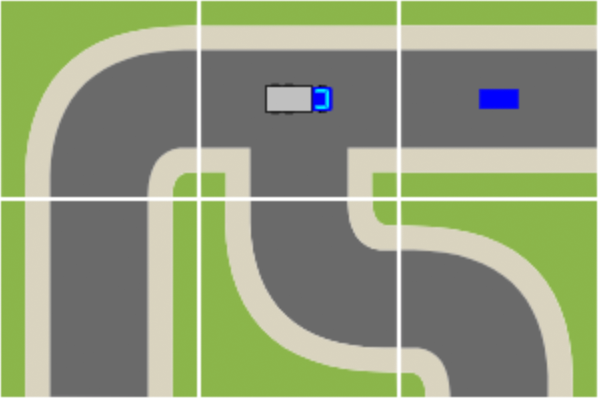
\includegraphics[width=\textwidth]{gfx/implementation-rendering-truck-position-diff-a.png}
    \caption{Haltepunkt auf der Mitte der Kachel}
    \label{fig:implementation:rendering:truck-position:diff:a}
  \end{subfigure}\hfill
  \begin{subfigure}[b]{0.45\textwidth}
    \includegraphics[width=\textwidth]{gfx/implementation-rendering-truck-position-diff-b.png}
    \caption{Haltepunkt auf der Kante der Kachel}
    \label{fig:implementation:rendering:truck-position:diff:b}
  \end{subfigure}\hfill
  \caption{Haltepunkte des Lastwagen im Spielfeld}
  \label{fig:implementation:rendering:truck-position:diff}
\end{figure}

\subsection{Animationsschritte}
\label{sec:implementation:rendering:animation}

Durch Animationen kann das Benutzererlebnis noch einmal deutlich aufgewertet werden. Zwischen den Positionen des Lastwagen wird daher zeitlich interpoliert. Eine wichtige Grundlage dafür wurde mit der Welt-Objektstruktur bereits geschaffen \tref{sec:implementation:structure}: Jede Operation erzeugt einen neuen Zustand, der gespeichert wird. Dieses Vorgehen macht es leicht zwischen dem aktuellen und dem vorherigen Zustand zu interpolieren.

Zur Darstellung einiger Operation wir eine gewisse Zeit benötigt. So ist für die Operation des vorwärts Fahren, ein Zeitschritt festgelegt, beim Setzten eines Blinkers kann die verbrauchte Zeit jedoch vernachlässigt, daher wird diese Operation mit null Zeitschritten bewertet. Die tatsächliche Zeit, die ein Zeitschritt verbraucht, kann festgelegt werden. Dadurch ist es möglich die Zeit (z.B. für die Auswertung von Testfällen) kleiner zu stellen und dadurch die Animationen schneller laufen zu lassen. Als Standardeinstellung hat sich die dauer von einer Sekunde für einen Zeitschritt als passend erwiesen.

Auch sind die Zeitschritte für die Berechnung der Ampelphasen relevant. Für Ampeln kann die Dauer der Rot-, bzw. Grünphase in Zeitschritten festgelegt werden. Eine Ampel mit einer Rotphase von einem Zeitschritt sowie einer Grünphase von ebenfalls einem Zeitschritt wir nun nach jeder Vorwärtsbewegung oder Aufruf des Warten-Befehls, umspringen. Jedoch nicht beim Wechsel der Blinkerseite. 

Um der Animationszeit im Programmablauf gerecht zu werden stellt, die \inlinec{World}-Klasse neben der \inlinec{command}-Methode auch noch die Methode \inlinec{commandAsync} bereit, die als asynchrone Funktion definerit ist und ein \inlinec{Promise} zurück gibt, welches Erfüllt wird, sobald die für diesen Befehl vorgesehene Zeit abgelaufen ist. Die MDN-Web-Dokumentation (Mozilla Developer Network) beschreibt asynchrone Funktionen wie folgt:

\begin{quote}
  "Eine asynchrone Funktion arbeitet außerhalb des Kontrollflusses, und teilt ihr Ergebnis durch ein unausgedrücktes, in die Ereignisschleife eingefügtes \inlinec{Promise} mit. Die Gestalt des Codes bei einer asynchronen Funktion ähnelt allerdings der der standardmässigen synchronen Funktionen. [...] Eine \inlinec{async} Funktion darf einen \inlinec{await} Ausdruck enthalten, der die Ausführung der Funktion anhält. Die Funktion wartet auf den zurückgegebenen ("resolved") Wert des \inlinec{Promise}, das der \inlinec{await} Ausdruck erzeugt, worauf die Funktion ihre Arbeit wieder aufnimmt."~\cite{mdn-async-function}
\end{quote}

Wärend die Nutzung von asynchronen Funktionen also technisch im Prinzip der Nuztung von Promises entspricht, vebessern sie die Lesbarkeit deutlich. Dies ist eine Eigenschaft, die besonders für den vom Compiler generierten Code \tref{sec:implementation:program:evaluation} nützlich ist und dort zum Einsatz kommt. Im generierten Code wird aus diesem Grund jedem Befehlsaufruf ein \inlinec{await} vorangestellt. Außerdem werden auch alle benuzterdefinierte Prozeduren als asynchrone Funktionen definiert.

In Abschnitt \ref{sec:implementation:program:evaluation} wurde bereits angedeutet, dass für die Ausführung des generierten Codes eine Funktion mit dem \inlinec{AsyncFunction}-Kontruktor erzeugt wurde. Im gegensatz zu \inlinec{Function} ist \inlinec{AsyncFunction} kein globales Objekt und kann auf etwas umständliche Weise durch die Ausführung des in \figreft{fig:implementation:rendering:animation:async-function} dargestellten Codes erhalten werden~\cite{mdn-async-constructor}.

\TODO{TypeScript-Compiler-Problem, Anforderung an den Browser}

\begin{figure}
  \lstinputlisting{snippets/implementation-rendering-animation-async-function.js}
  \caption{Erhalten des \inlinec|AsyncFunction|-Objekt~\cite{mdn-async-constructor}}
  \label{fig:implementation:rendering:animation:async-function}
\end{figure}

%************************************************
% Integration
%************************************************
\section{Integration}
\label{sec:implementation:integration}

Um mit möglichst wenigen Abhängigkeiten und dadurch der Möglichkeit mit geringerem Zeitaufwand verschiedene Ansätze ausprobieren zu können, wurde zunächst mit der Entwicklung eines Prototypen auf einer "grünen Wiese" begonnen. Auch wenn der Prototyp als Angular-Anwendung aufgesetzt wurde, erfolgte der Großteil der Entwicklung erfolge außerhalb dieser Umgebung. Nachdem der ursprüngliche Ansatz der Darstellung mittels SVG-Grafiken verworfen wurde und die Darstellung auf Canvas-Rendering umgestellt wurde, sind die Objektstruktur, sowie der Renderer wurden völlig unabhängig von Angular, da sie von den von Angular bereitgestellten Strukturen nicht profitieren können. Diese Klassen konnten so ohne Anpassungen in die Umgebung von BlattWerkzeug übernommen werden. Lediglich die rudimentäre Benutzeroberfläche des Prototypen \figref{fig:implementation:integration:prototype} wurde mit Hilfe von Angular umgesetzt, für die Integration in BlattWerkzeug jedoch nicht mehr benötigt.

\begin{figure}
  \centering
  \includegraphics[width=0.35\textwidth]{gfx/implementation-integration-prototype.png}
  \caption{Bildschirmfoto der UI des Prototyp}
  \label{fig:implementation:integration:prototype}
\end{figure}

\subsection{Angular-Service}
\label{sec:implementation:integration:ng-service}

\TODO{Auslagerung der Welt in einen Service}

\subsection{Renderer}
\label{sec:implementation:integration:renderer}

\TODO{Renderer}

\subsection{Fortschrittsmeldungen}
\label{sec:implementation:integration:progress}

\TODO{Rückmeldung über den Fortschritt des Programm zur Anzeige im Drag \& Drop-Editor => Ausblick?}
